% status: 0
% chapter: TBD

\title{Presto: Distributed SQL Query Engine for Big Data}


\author{Ankita Alshi}
\affiliation{%
  \institution{Indiana University Bloomington}
  \city{Bloomington}
  \state{Indiana}
  \postcode{47404}
  \country{USA}
}
\email{aralshi@iu.edu}

\author{Gregor von Laszewski}
\affiliation{%
  \institution{Indiana University}
  \streetaddress{Smith Research Center}
  \city{Bloomington} 
  \state{IN} 
  \postcode{47408}
  \country{USA}}
\email{laszewski@gmail.com}


% The default list of authors is too long for headers}
%\renewcommand{\shortauthors}{G. v. Laszewski}


\begin{abstract}
Presto is a SQL query engine developed specially for interactive analytics. It
focuses on large commercial data warehouses with capacity of gigabytes to
petabytes. It is open source and used for distributed systems. It is compatible
with relational as well as NoSQL data sources such as Cassandra and
Hive~\cite{hid-sp18-502-Presto}.

It is being used by big organizations like Facebook to run interactive queries
against their large data warehouses. The main advantage of using Presto is that
it allows to perform analytics on data from different data sources using single
query. This allows data to be combined across organizations without extra
overhead of separate queries for each data source~\cite{hid-sp18-502-Presto}.
\end{abstract}

\keywords{hid-sp18-502, SQL, Hadoop, Map-reduce, Big data}


\maketitle


\section{Introduction}

All the big organizations usually have large data warehouses and different data
sources which needs to be well integrated to provide efficient use of them. Now
a days there is a high demand of interactive and quick query processing for
analytical processes. It is become necessary to use SQL on Hadoop so that
larger group of organizations can use the Hadoop on commodity clusters to
fulfill their technology need. Presto is one such open source SQL engine that
provides the functionality to interact with distributed database with very
low latency.
Hive can also be used for running SQL queries on big data systems but it takes
longer time to execute the queries. Fast query execution of presto is achieved
by complete pipelining of query execution. Also Presto is a in memory SQL query
execution in engine which means that data on which query is executed resides in
main memory of the nodes. This eliminates the time required to access that data
from the disk. disadvantage of in-memory query execution is that it is not
fault tolerant as the intermediate query results are not stored on any
non-volatile storage device. Also there is a restriction on the size of the
query as not all the data can be stored in memory of the nodes. So large
queries which require data more than the size of the main memory would not be
executed successfully.
Presto is implemented in Java as it is easy to integrate it with other systems
and maintain the code as well.

\section{Architecture}

Presto is designed to provide speed for analytical queries.
Figure~\ref{f:architecture} explains architecture of presto and control flow.
Client queries are sent to the coordinator server. It first parses the SQL query
 using Metadata APIs. The parsed query is goes through the planning stage where
 its execution is planned such that it can be executed in pipeline. After that
 coordinator uses data location APIs to schedule the tasks to run on different
 worker nodes such that each worker node is execute query on its local data
 stored in main memory. Once tasks are schedule all the worker nodes execute
 each task in pipelined mode. The query is divided into stages and data is
 passed on from one stage to another as it is ready. This ensures that at a time
  multiple queries are executed by each node providing additional level of
  parallelism to achieve faster results. Pipelining is done across the network
  such that any available node can execute different stages. The data transfer
  is from main memory to main memory so it takes less time. when the result are
  ready worker node sends it back to the client. Coordinator server keeps
  monitoring the query execution.

\begin{figure}[!ht]
  \centering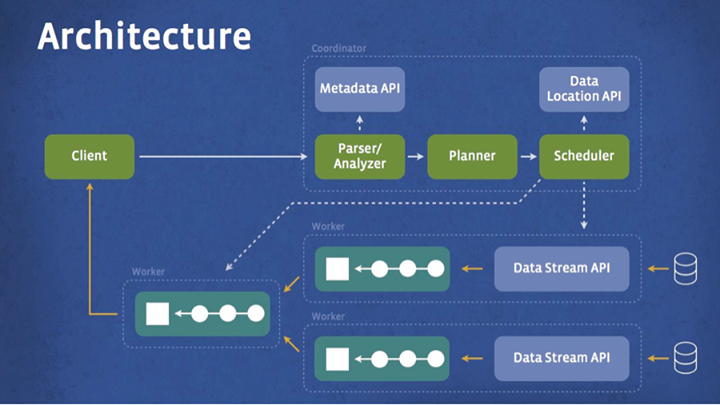
\includegraphics[width=\columnwidth]{image/presto-architecture.png}
  \caption{Presto Architecture}\label{f:architecture}
\end{figure}

\section{Concepts}
\subsection{Server Types}
There are two types of servers in presto architecture- Coordinator and Worker.
Both the types of servers are different set of responsibilities that they work
towards.
\subsubsection{Coordinator}
Presto coordinator server can be considered by main backbone of the system.
Coordinator server responsible for managing the worker server present in presto
setting. All the client queries are routed to coordinator server. Coordinator
server contains all the information of the worker servers, where they are
located and the data that they locally store. This information is used wisely
by the server to plan the query into task and to schedule these tasks across the
nodes on the network such that data required for executing these task is either
present locally or very close to the worker server. Additionally Coordinator
server also keeps track of query execution once the worker nodes starts
processing it.
Coordinator server parse the SQL query and creates a logical model out of it
such that it can be executed in series to stages. These stages are nothing but
the task which are executed on distributed worker nodes available in the
cluster. Each Presto installation needs at least one Coordinator server.

\subsubsection{Worker}
Worker server is mainly responsible for processing the queries assigned to it
by the coordinator. Worker node fetches the data required for the query
processing from connectors or other worker nodes. When a new presto worker node
starts up, it informs the coordinator server in the presto installation. This
way the coordinator server gets to know that new worker is added to the
installation and can be considered to schedule tasks to run on it.
Worker node executes the query as it is planned by the coordinator. Intermediate
results generated by worker nodes are passed on to other worker node on which
the next execution stage is scheduled. Final results generated by worker node is
sent back to the coordinator server which sends it back to the client.

\subsection{Data Sources}
Presto id designed to work with different types of data sources. Connectors are
used in order to run SQL query against all the types data sources. Connectors
are very similar to database drivers, they provide set of APIs to connect to
that database. Presto contains connectors to connect to Hive, HBase, relational
databases and NoSQL data sources as well. Presto keeps catalogs to resolve the
queries. Catalogs are used to store the schema for different connectors.
Catalogs are used to reference the connectors. Schema is nothing but way of
organizing the data in different data sources. schema for a relational database
is table whereas for a NoSQL database is a document. Catalogs and schema are
used to defined traditional set of tables against which the SQL queries can be
processed.

\subsection{Query Execution}
Client sends SQL statements to the coordinator. This SQL statement can not be
executed as it is by the worker. Coordinator server parses this statement into
distributed query plan. Distributed query plan can be visualized as a tree with
leaf nodes processing small tasks and parent of those nodes executing aggregated
functions on their results. At the end root node aggregates results of all
nodes in the tree to create the final output.
Distributed query plan is created as a set of interconnected stages. Data flows
from one stage to another. Each stage might involve in retrieving data from
different data sources using connectors. At the end of each stage an
intermediate output is generated. Instead of running a complete stage on one
node,the stage is further divided into tasks and these tasks are scheduled to
run on worker nodes.

\section{Use Case}

\section{Conclusion}



\begin{acks}

  The authors would like to thank Dr.~Gregor~von~Laszewski for his
  support and suggestions to write this paper.

\end{acks}

\bibliographystyle{ACM-Reference-Format}
\bibliography{report} 

